%\textit{
 %   \textbf{
  %      The following section formatting is optional, you can also define sections as you deem fit.
   %     \\
    %    Focus on what future researchers or practitioners would find useful for reproducing or building upon the paper you choose.\\
     %   For more information of our previous challenges, refer to the editorials \cite{Sinha:2022,Sinha:2021,Sinha:2020,Pineau:2019}.
    %}
%}

\section{Introduction}
The trend towards using ever-more complex machine learning models in the field of Computer Vision has led to improved accuracy at the cost of interpretability. 
Most state-of-the-art models are inherently opaque, making understanding their inner dynamics and decision-making processes difficult. 
This has motivated the emerging research area of explainable AI \cite{das2020opportunities}, with a strong focus on explaining the classification of images. Numerous explanation methods, like Smoothgrad~\cite{smilkov2017smoothgrad} or LIME~\cite{ribeiro2016lime}, have been developed for image classifiers.
These methods all operate in the pixel domain, producing pixel-sparse or jittery explanations. 

Challenging this approach, the authors of~\cite{cartoonX} proposed CartoonX; a novel, model-agnostic explanation method for image classifiers that operates in the wavelet domain.
This paradigm shift is motivated by the idea that demanding sparsity in the wavelet domain introduces piece-wise smooth explanations, i.e., asking the question \textit{What is the piece-wise smooth part of the input signal that leads to the model decision?}~\cite{cartoonX}.
CartoonX generates explanations by applying the rate-distortion explanation (RDE) framework (originally proposed by~\cite{rdeOriginal} and extended by~\cite{rdeExtend}) in the wavelet domain of an image.
RDE is an optimization problem that enforces maximum sparsity with minimum distortion in the model's output.
This is achieved by optimizing a deletion mask applied to the image coefficients, thus marking relevant components.
In the conventional setting, Pixel RDE enforces sparsity on (super-)pixels.
In the case of CartoonX, RDE is used to enforce sparsity across the wavelet coefficients.

In this contribution, we aim to reproduce the results of the CartoonX paper and perform an additional experiment to examine the authors' main claims. Moreover, an extension is proposed to improve the runtime of CartoonX. 

The remainder of this paper is organized as follows: Section \ref{sec:claims} presents the scope of this reproducibility study and the methodology is outlined in Section \ref{sec:meth}. In Section \ref{sec:results}, the results are presented and discussed. Section \ref{sec:over} discusses different aspects of the reproducibility effort. Lastly, in Section \ref{sec:conclusion}, a conclusion is given. 

\section{Scope of Reproducibility}
\label{sec:claims}

In this reproducibility study, we examine the original authors' claims:
\begin{itemize}
\setlength\itemsep{-0.1em}
    \item CartoonX extracts relevant piece-wise smooth parts of the image, resulting in more straightforward explanations.
    \item CartoonX achieves lower distortion in the model output while using fewer coefficients than other state-of-the-art methods.
    \item CartoonX is model-agnostic.
\end{itemize}

% Explain first two claims --> with the quantititave and    qualitative?  
The explanations provided by CartoonX are qualitatively evaluated (i.e., manually compared and interpreted) to examine the first claim. 
To investigate whether CartoonX achieves lower distortion in the model output, the distortion of the different methods is compared. This is referred to as the quantitative evaluation. 

The original authors used two CNNs in their experiments to investigate their claim of model agnosticism.
We extend their experiments by running CartoonX with a Vision Transformer (ViT). The results of CartoonX with a ViT are compared to an attention map of the Transformer model.
Attention maps have been used in other works to explain model decisions~\cite{chefer2021transformer}, serving as a basis for the cross-validation of CartoonX.

%Furthermore, we demonstrate that improving CartoonX's runtime via enhanced initialization techniques of the deletion mask is difficult.
The original authors suggested to train a neural network to predict a good initialization of the deletion mask for arbitrary images of the target distribution with the intention of significantly reducing CartoonX's runtime. This should ideally lead to faster convergence. 
Due to the computational cost of generating sufficient training data, two different heuristical strategies were assessed.
%Our results indicate that simple feature engineering might be insufficient to achieve competitive runtimes.
%As the original authors suggested before us, it may be necessary to use more complex methods such as a neural network to find a good initialization. Such a network could be trained to suggest an initial deletion mask for arbitrary images of the target distribution.

Summarizing, the main contributions of this publication are:
\begin{itemize}
\setlength\itemsep{-0.1em}
    \item Examining the first two claims of the original authors by reproducing the experiments and qualitative and quantitative evaluating the results.
    %\item Re-evaluating the performance of CartoonX qualitatively and quantitatively.
    \item Applying CartoonX with a ViT to investigate the model agnosticism claim.
    \item Exploring using simple heuristics for initialization to improve runtime.
\end{itemize}

%Each experiment in Section~\ref{sec:results} will support (at least) one of these claims, so a reader of your report should be able to separately understand the \emph{claims} and the \emph{evidence} that supports them.

%\jdcomment{To organizers: I asked my students to connect the main claims and the experiments that supported them. For example, in this list above they could have ``Claim 1, which is supported by Experiment 1 in Figure 1.'' The benefit was that this caused the students to think about what their experiments were showing (as opposed to blindly rerunning each experiment and not considering how it fit into the overall story), but honestly it seemed hard for the students to understand what I was asking for.}

\section{Methodology}\label{sec:meth}
%Explain your approach - did you use the authors' code, or did you aim to re-implement the approach from the description in the paper? Summarize the resources (code, documentation, GPUs) that you used.

The original authors provide a publicly available, well-documented, and cleanly written codebase,\footnote{\url{https://github.com/skmda37/CartoonX}} containing all necessary implementations to produce CartoonX and Pixel RDE explanations. Nonetheless, neither an implementation for their quantitative evaluations nor a reference to the original images was published, complicating the reproducibility effort. The authors' implementation was used as a baseline and adapted to accommodate the outlined extensions and it was supplemented with the quantitative experiments. We consulted with the authors to verify the correctness of our interpretation. The extended open-source repository is made publicly available.\footnote{\url{https://github.com/JonaRuthardt/MLRC-CartoonX}}

\subsection{CartoonX} \label{sec:cartoonx}
CartoonX~\cite{cartoonX} is a rate-distortion-based explanation method for image classifiers operating in the wavelet domain to identify the components (i.e., wavelet coefficients) of an image that are most decisive for the model's prediction. 

For this, a given image is transformed into its wavelet representation by applying the Discrete Wavelet Transform (DWT).
Out of the resulting DWT coefficients $h$ that represent the image in wavelet space, the least relevant components are masked. This is done by iteratively learning a mask $s$ that minimizes a distortion metric while encompassing minimal components. The sparsity is enforced by applying the $\ell_1$-norm on the mask's values and controlled using an additional parameter\footnote{Parameter $k$ refers to the number of pixels, while $\lambda$ refers to the sparsity level. We will treat them as a single parameter to retain consistency with the original authors.} $\lambda k$ by which this loss component is multiplied. Starting with an all-ones initialization, the mask's values are continuously decreased for wavelet components that contain little classification decisive information. %Adam~\cite{kingma2014adam} was used as an optimizer.
At every iteration, a batch of $L$ adaptive Gaussian noise samples \sloppy${v^{(1)},\,...,\,v^{(L)}}$ is drawn.
With these samples, the obfuscations \sloppy${y^{(1)},\,...,\,y^{(L)}}$ are computed as \sloppy${y^{(i)} = \text{DWT}^{-1}(h\;\odot s + (1-s) \odot v^{(i)})}$.
Therefore, less relevant components with mask values close to $0$ will be (partially) replaced by noise. The efficacy of the mask is ascertained by computing the distortion $\hat{D}(x, s, \Phi)$ as the average squared distances of the post-softmax originally predicted class probabilities of the original image $x$ and the set of obfuscations.
Together with the sparsity constraint, the loss objective emerges as \sloppy${l(s) = \hat{D}(x, s, \Phi) + \lambda \|s\|_1}$.

The explanation is ultimately obtained by applying the learned mask to the image's wavelet coefficients and converting the resulting representation back into pixel space as a grayscale image. This results in a piece-wise smooth image explaining the model's decision by highlighting relevant areas for each image. For a more comprehensive and conclusive background on the rate-distortion framework and the exact implementation of CartoonX, we refer back to Sections 3 to 5 in~\cite{cartoonX}. 

% It enforces sparsity by applying a continuous mask $s$ on the DWT coefficient of the image (i.e., in wavelet space) instead of on the images' pixels directly (i.e., in pixel space). The values of mask $s$ range from 0 to 1, 1 meaning not masked at all and 0 meaning completely masked. For every individual image, this mask is learned, combined with the image and converted back to pixel space. 

%Specifically, first an image is converted to the wavelet domain through the Discrete Wavelet Transform (DWT), using the Daubechies 3 (db3) wavelet system with zero-padding and 5 scales, resulting in DWT coefficients $h$. Then, the mask $s$ is initialized, with the default initialization being with ones. Moreover, the sparsity level is initialized with the default $\lambda k=20$. Then for a predefined number of steps (here N = 2000), this mask $s$ is optimized using the Adam Optimizer \cite{kingma2014adam} with a learning rate of 0.001. At every step, a batch of L=64 adaptive Gaussian noise samples $v^{(1)}, ...v^{(L)}$ are drawn and with those the obfuscations $y^{(1)}, ...y^{(L)}$ are computed with $y^{(i)} = IDWT(h*s + (1-s)*v^{(i)})$. With those obfuscations, the distortion $\hat{D}(x, s, \Phi)$ is computed by taking the squared distance in the post-softmax probability of the predicted label for the input image $x$ and for the obfuscation $y^(i)$ and averaging over all computed distortions for the $L$ number of obfuscations. 

 %The loss function used for the optimizer is $l(s) = \hat{D}(x, s, \Phi) + \lambda k \|s\|_1$ where $\lambda k \|s\|_1$ refers to the level of sparsity. This way, CartoonX learns the best mask by minimizing the distortion between the original image and the image combined with the learned mask while also maximizing the sparsity of $s$. After training, the mask $s$ is combined with the images' DWT coefficients and converted back to pixel space with the IDWT, resulting in a piece-wise smooth image explaining the model decision for each individual image.

%For the complete background on the rate-distortion (RDE) framework and on the exact implementation of CartoonX, we refer back to sections 3, 4 and 5 of the original paper on CartoonX~\cite{cartoonX}. 

\subsection{Model descriptions}
%Include a description of each model or algorithm used. Be sure to list the type of model, the number of parameters, and other relevant info (e.g. if it's pre-trained).

To reproduce the results from the original paper, we also used a pre-trained MobileNetV3-Small~\cite{mobilenetv3} (Top-1 accuracy $67.7\%$; $1.8$M parameters).
It was additionally used to test for the speed-up effects of different mask initialization techniques.
Furthermore, a pre-trained Transformer-based classifier in the form of DeiT-tiny~\cite{efficientVisionTransformer} (Top-1 accuracy $72.2\%$) was examined.
%With an emphasis on data and runtime efficiency comprising a comparatively low 5 million parameters, this model is more suitable for the employed post-hoc explanation approach that is primarily constrained by the duration of model backward passes.
This particular ViT was chosen due to its comparatively few 5M parameters, thus, behaving runtime efficiently.
All models used in this study and the original paper were pre-trained on ImageNet1K.


%Instead of using a VGG16, we focused our attention on using a pretrained vision transformer, called DeiT-tiny~\cite{efficientVisionTransformer} (Top-1 accuracy 72.2\%).
%It is an efficient transformer architecture, with only 5 million parameters.
%Therefore, it is well suited for our experiments, which need many backwards passes through the network while working with limited resources.



\subsection{Datasets}
%For each dataset include 1) relevant statistics such as the number of examples and label distributions, 2) details of train / dev / test splits, 3) an explanation of any preprocessing done, and 4) a link to download the data (if available).

For all experiments, we used the same random sub-set of $100$ images of $100$ distinct but randomly selected classes from ImageNet.\footnote{\url{https://github.com/EliSchwartz/imagenet-sample-images}}
In line with the original publication, the images were resized to $256 \times 256$ pixels. Only for experiments involving the Transformer-based model (i.e., the \textit{Model Agnosticism Experiment}) were the images resized to $224\times224$ pixels to ensure model compatibility.

\subsection{Experimental setup and code}
%Include a description of how the experiments were set up that's clear enough a reader could replicate the setup. 
%Include a description of the specific measure used to evaluate the experiments (e.g. accuracy, precision@K, BLEU score, etc.). 
%Provide a link to your code.

In order to verify and extend the claims made in \cite{cartoonX}, three different experimental setups are proposed and specified in this Section.  

% The quantitative evaluation of the proposed method is based on the calculation of the \textit{distortion} metric introduced in Section \ref{sec:cartoonx}. Additionally, a thorough qualitative assessment was conducted. 

\subsubsection{Reproducibility Experiment}\label{exp1}

%The first two claims that the proposed method demonstrates an improved interpretability and a less distorted representation while requiring fewer components can be substantiated through both quantitative and qualitative assessments. 
The reproduction of the experiments consists of two parts. The qualitative experiment, corresponding to the claim that CartoonX is qualitatively better to interpret, and the quantitative experiment, corresponding to the claim that CartoonX achieves lower distortion while using fewer coefficients.
%This objective is met by attempting to reproduce the principal experiments initially proposed. 
Both quantitative and qualitative experiments were evaluated akin to the original paper.%publication.
%That is, the model was parameterized with the same hyperparameters and setup as the original authors \cite{cartoonX}. The hyperparameters and its values are specified in the next Section. 

For the qualitative experiment, explanations for the $100$ images with both the CartoonX and Pixel RDE methods were created. The most insightful and interesting explanations are used to highlight and discuss the interpretability of CartoonX compared to Pixel RDE. To increase transparency and mitigate potential selection biases, all results underlying the qualitative evaluations are made publicly available in our repository. 

The quantitative experiment consists of three different subexperiments.
%For the first two subexperiments, the same masks that are used to create the 100 explanations for the qualitative experiment are used.
In the first two subexperiments, the optimized masks for the $100$ explanations of the qualitative experiment are used.
For the first subexperiment, all components are randomized with adaptive Gaussian noise, except for an iteratively increasing fraction of the most relevant components, (i.e., the highest mask values).
Conversely, in the second experiment, the most relevant components are randomized. Finally, the third subexperiment examines the distortion and non-sparsity (the two loss terms) for varying $\lambda k$.

% This experimental baseline was run using different $\lambda k$'s for both explanation approaches in powers of two ranging from $2^2$ to $2^6$ to allow conclusions on model-specific sparsity requirements to be drawn.

\subsubsection{Model Agnosticism Experiment}\label{exp2}
To examine the claim that CartoonX is model-agnostic, the ViT DeiT-tiny \cite{pmlr-v139-touvron21a} was integrated into the CartoonX framework. For all $100$ images, three different explanations were created: a CartoonX explanation for both the ViT as well as the CNN, and the attention rollout \cite{abnar2020quantifying}. The latter method linearly combines the attention weights throughout the layers of the vision transformer. More specifically, at each layer, it merges the attention at each position with the attention at each position of the previous layers. To account for the multiple attention heads, we take an average of all heads. The implementation by \cite{vitexplain_repo} is used to create the attention rollout.
Moreover, the quantitative evaluation for this experiment is set up analogously to the quantitative evaluation for the reproducibility experiment.

\subsubsection{Runtime Efficiency Experiment}\label{exp3}
To improve runtime, we explore using simple heuristics for initializing the deletion mask. Two different strategies were tested.
In the first strategy, we use an efficient preoptimization algorithm, which iteratively decreases the initial mask from $1$ to $0$ in one-percent increments until the network predicts a new class.
This pre-convergence criterion was chosen heuristically.
Up until this point, the gradients are still largely useful.
%After a new class is predicted, it was found to be harder to recover significant wavelet coefficients that are already masked out.
The second strategy uses a binary foreground mask as an initialization, with $1$ for wavelet coefficients corresponding to foreground regions and $0$ for those corresponding to background regions.
The main idea is that the network primarily uses the foreground to predict the class.
Consequently, it is the part of the image containing most of the relevant frequencies needed to explain the model's decision.
%A proposition put forward as an possible improvement in the original publication is to reduce the time and resource requirements associated with the creation of an explanation. By virtue of being a post-hoc explanation method, the generation of an explanation for a given image involves an extensive and computationally expensive optimization procedure making it costly or even infeasible for large-scale explanation generation. 
%In order to obtain expressible gradients, it is necessary for the model to have sufficient confidence in its predictions. Consequently, perturbating the image with noise to the point where its content becomes unrecognizable to the model yields all-zero masks that were singularly optimized for the sparsity component and maximally distort the image. 
%To demonstrate the runtime efficiency improvement potential, a primitive initialization heuristic is proposed that iteratively and collectively lowers the initialization values of the mask while keeping the aforementioned restriction in mind. More precisely, the value of each mask component, initially starting at one, is gradually decreased in one percent increments until the model changes the class it would predict. This can be interpreted as the act of adding noise augmentations to the image until the point at which it becomes indistinguishable from other classes. Applying this pre-optimization step helps to ensure that adequate loss signals are still available while swaying most components more towards the value they will eventually converge towards (i.e., zero for most components due to the sparsity constraint). 
The efficacy of each of these approaches was evaluated based on the loss curves obtained during the actual optimization. Hence, it is possible to ascertain that the model converges towards approximately the same loss value and if it does so after fewer iterations.
We compared these strategies to a random initialization and the default all-ones initialization, as implemented by the original authors.


\subsection{Hyperparameters}
%Describe how the hyperparameter values were set. If there was a hyperparameter search done, be sure to include the range of hyperparameters searched over, the method used to search (e.g. manual search, random search, Bayesian optimization, etc.), and the best hyperparameters found. Include the number of total experiments (e.g. hyperparameter trials). You can also include all results from that search (not just the best-found results).

For all experiments, the default values for all hyperparameters -- as specified in \cite{cartoonX}, Section 5 -- were used.
Whenever the hyperparameters were not specified, we used the default values in the code provided by the original authors.
To choose a proper value for $\lambda k$ for the ViT, we did a qualitative search (see Appendix~\ref{ap:hyperparam} for details).
%We found $\lambda k=10$ to yield the best results.
For the attention rollout explanation, the attention heads were fused by taking the mean (as done in \cite{abnar2020quantifying}) and the discard ratio of $0.9$ is chosen, to focus on the highest attention values.
The following table gives an overview of the experimental setups used:
%If you take out the table, reintroduce the sentence "We found $\lambda k=10$ to yield the best results."

\begin{table}[htb]
\centering
\footnotesize
\begin{tabular}{c||c|c|c|c|c|c|c|c}
     %& \thead{$\lambda k$} & \thead{iterations} & \thead{batch size \\(adaptive Gaussian noise)} & \thead{optimizer} & \thead{learning rate} \\
     Experiment & CNN $\lambda k$ & ViT $\lambda k$ & P. RDE $\lambda k$ & iter. & b. size & optimizer & lr & init. mask\\
     \hline
    Reprod. & $20$ & N/A & $4$ & $2000$ & $64$ & Adam~\cite{kingma2014adam} & $10^{-3}$ & ones \\
    Agnost. & $20$ & $10$ & N/A & $2000$ & $64$ & Adam & $10^{-3}$ & ones\\
    Runtime & $20$ & N/A & N/A & $2000$ & $64$ & Adam & $10^{-3}$ & various\\
\end{tabular}
\vspace{-2mm}
\caption{\footnotesize Overview of hyperparameter settings used in our experiments.}
\label{tab:my_label}
\end{table}
\vspace{-6mm}

\subsection{Computational requirements}
%Include a description of the hardware used, such as the GPU or CPU the experiments were run on. 
%For each model, include a measure of the average runtime (e.g. average time to predict labels for a given validation set with a particular batch size).
%For each experiment, include the total computational requirements (e.g. the total GPU hours spent).
%(Note: you'll likely have to record this as you run your experiments, so it's better to think about it ahead of time). Generally, consider the perspective of a reader who wants to use the approach described in the paper --- list what they would find useful.

% I would just mention how many hours or compute each experiment (so 1, 2 and 3) took
% To run the experiments, we were provided with 20 hours of runtime on an Nvidia Titan RTX.
% Thereof we used x hours to recreate the quantitative analysis of Fig.~\ref{}, y hours to extent the results of CartoonX to vision transformers, and z hours testing various mask initializations.
% For the reproducibility experiment, X hours. 

% For the model agnosticism experiment, to run for 1 image, it takes 00:04:32 hours. Thus in total, 
% For only the ViT cartoonX, it takes 00:30:19  / 10 hours. 

Obtaining a singular explanation with the Mobilenet-based CartoonX and Pixel RDE approaches required $96$ and $75$ seconds on an NVIDIA Titan RTX, respectively. 
This equates to a total GPU walltime of $28.5$ hours to obtain all quantitative and qualitative results of 100 images with six different $\lambda k$. %(default and third subexperiment).
This is proportional to the reported times in \cite{cartoonX}.
%To produce an explanation for a single image with the CNN CartoonX and Pixel RDE with the aforementioned hyperparameters, Y minutes are needed on an Nvidia Titan RTX. This is (?) in line with the reported time of the orignal authors. To reproduce the qualitative and quantitative analysis (Section \ref{sec:repro}), 100 images have to be explained with 6 different settings of $\lambda k$. This results in X hours of runtime. 
Furthermore, the creation of all relevant explanations for the model agnosticism experiment requires $272$ seconds per image. Thus, for this whole experiment, $7.5$ hours of runtime were used. Finally, to test various mask initializations, $2.3$ hours were used. The overall GPU utilization during this study amounted to approximately $38.4$ hours. 


\section{Results and Discussion}
\label{sec:results}
%Start with a high-level overview of your results. Do your results support the main claims of the original paper? Keep this Section as factual and precise as possible, reserve your judgement and discussion points for the next "Discussion" Section. 

%We perform a quantitative analysis of the results of CartoonX and compare them to Pixel RDE and show that CartoonX uses fewer coefficients. Furthermore, we show that CartoonX can be applied to vision transformers and that in many cases the resulting explanations resemble the attention mask of the transformer model. We examine different initialization strategies for the deletion mask, including a preoptimization algorithm, with the goal of improving the runtime of CartoonX.

We performed a qualitative and quantitative analysis of the results of CartoonX and compared them to Pixel RDE.
Furthermore, CartoonX's performance on ViTs was evaluated and the results were compared to the corresponding attention masks.
Lastly, different initialization strategies for the deletion mask, including a preoptimization algorithm intended to improve the runtime of CartoonX, were examined.

\subsection{Results reproducing original paper} \label{sec:repro}
%For each experiment, say 1) which claim in Section~\ref{sec:claims} it supports, and 2) if it successfully reproduced the associated experiment in the original paper. 
%For example, an experiment training and evaluating a model on a dataset may support a claim that that model outperforms some baseline.
%Logically group related results into sections. 

\subsubsection{Qualitative Reproducibility Experiment}
%CartoonX explains a decision by extracting the piece-wise smooth parts of the image responsible for it.

%\begin{figure}
%    \centering
%    \includegraphics[width=55mm]
%    {images/pirate.png}
%    \caption{CartoonX generates piece-wise smooth explanations. Pixel RDE produces pixel sparse explanations.}
%    \label{fig:piece-wise_smooth_ex}
%\end{figure}

The original authors claimed that CartoonX extracts relevant piece‐wise smooth parts of the image, resulting in more intuitive explanations.
In Fig.~\ref{fig:qual_comp} we present a selection of explanation comparisons between CartoonX and Pixel RDE.
%Fig.~\ref{fig:piece-wise_smooth_ex} illustrates a sample comparison between explanations of CartoonX and Pixel RDE.
Pixel RDE produces pixel-sparse explanations.
%of the pirate ship.
Conversely, CartoonX introduces sparsity in the wavelet domain, blurring out irrelevant areas of the image.
%Note how background features blur into non-existence, while within the areas of the ship the presence of high frequencies is visible. 
These characteristics are what the notion of piece-wise smooth areas refers to.

\begin{figure}
    \centering
    \begin{tabular}{@{}c@{}}
        \includegraphics[width=50mm]{images/cartoonx_better.png}
    \end{tabular}
    \hspace{5mm}
    \begin{tabular}{@{}c@{}}
        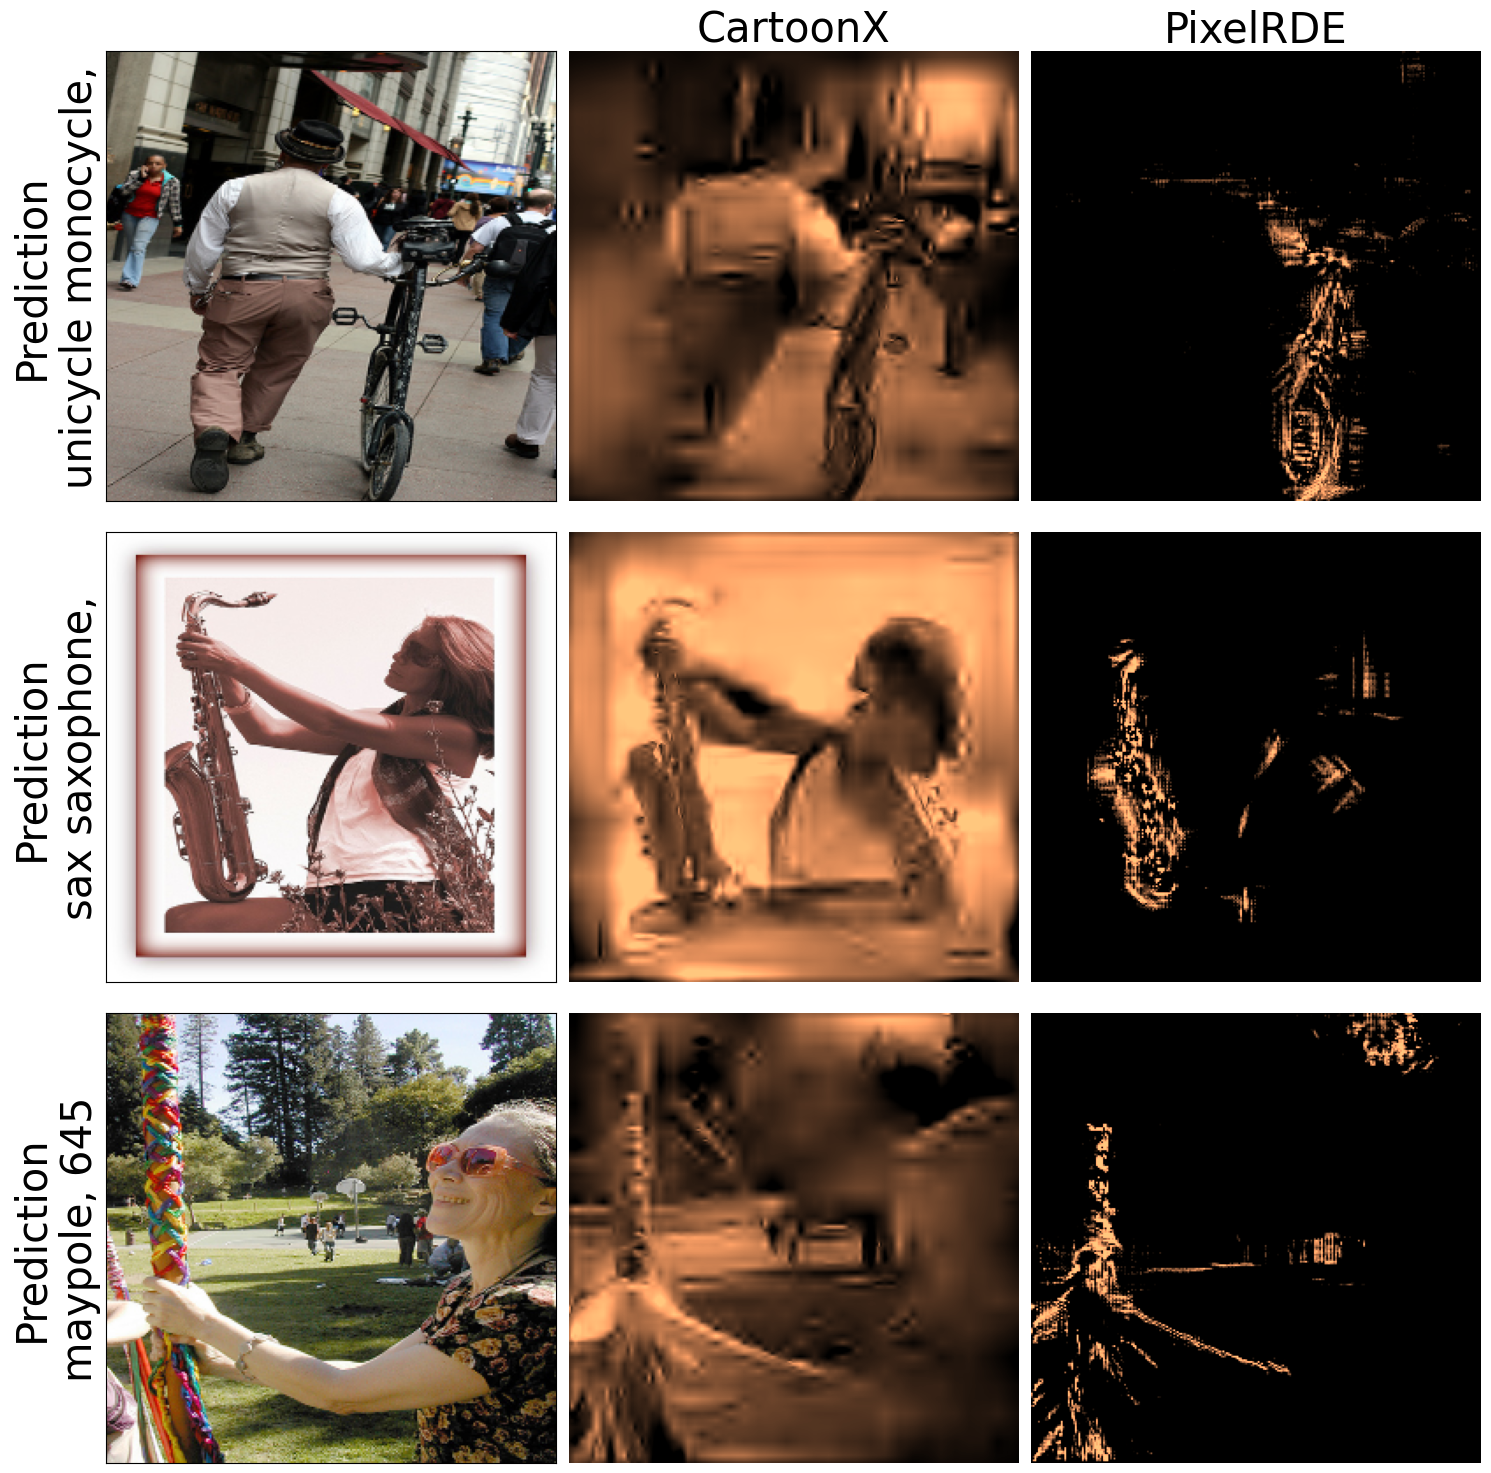
\includegraphics[width=50mm]{images/rde_better.png}
    \end{tabular}
    \caption{Examples of images where CartoonX produces subjectively better explanations (left) and examples of images where Pixel RDE produces subjectively better explanations (right).}
    \label{fig:qual_comp}
\end{figure}

Fig.~\ref{fig:qual_comp} highlights selected samples where either CartoonX outperforms Pixel RDE (left) or vice-versa (right).
Here, \textit{outperform} refers to the subjective, qualitative evaluation of the results.
In the left images, the explanations provided by Pixel RDE are sparse and hard to interpret.
Sometimes irrelevant parts of the background have also been marked.
CartoonX conserves the shape and, to some degree, the texture of the relevant parts of the image.
In the right images, all objects themselves are identified as the principal explanations by Pixel RDE.
CartoonX also considers the people using these things and part of the background as an explanation.
Nonetheless, overall it was much easier to find examples of CartoonX outperforming Pixel RDE than the other way around.
Even in the latter case, CartoonX still provides predominantly reasonable explanations.
%Using larger values for $\lambda k$ can also improve the quality of these results.

\begin{figure}
    \centering
    \begin{tabular}{@{}c@{}}
        \includegraphics[width=50mm]{images/model_bad_x_good.png}
    \end{tabular}
    \hspace{5mm}
    \begin{tabular}{@{}c@{}}
        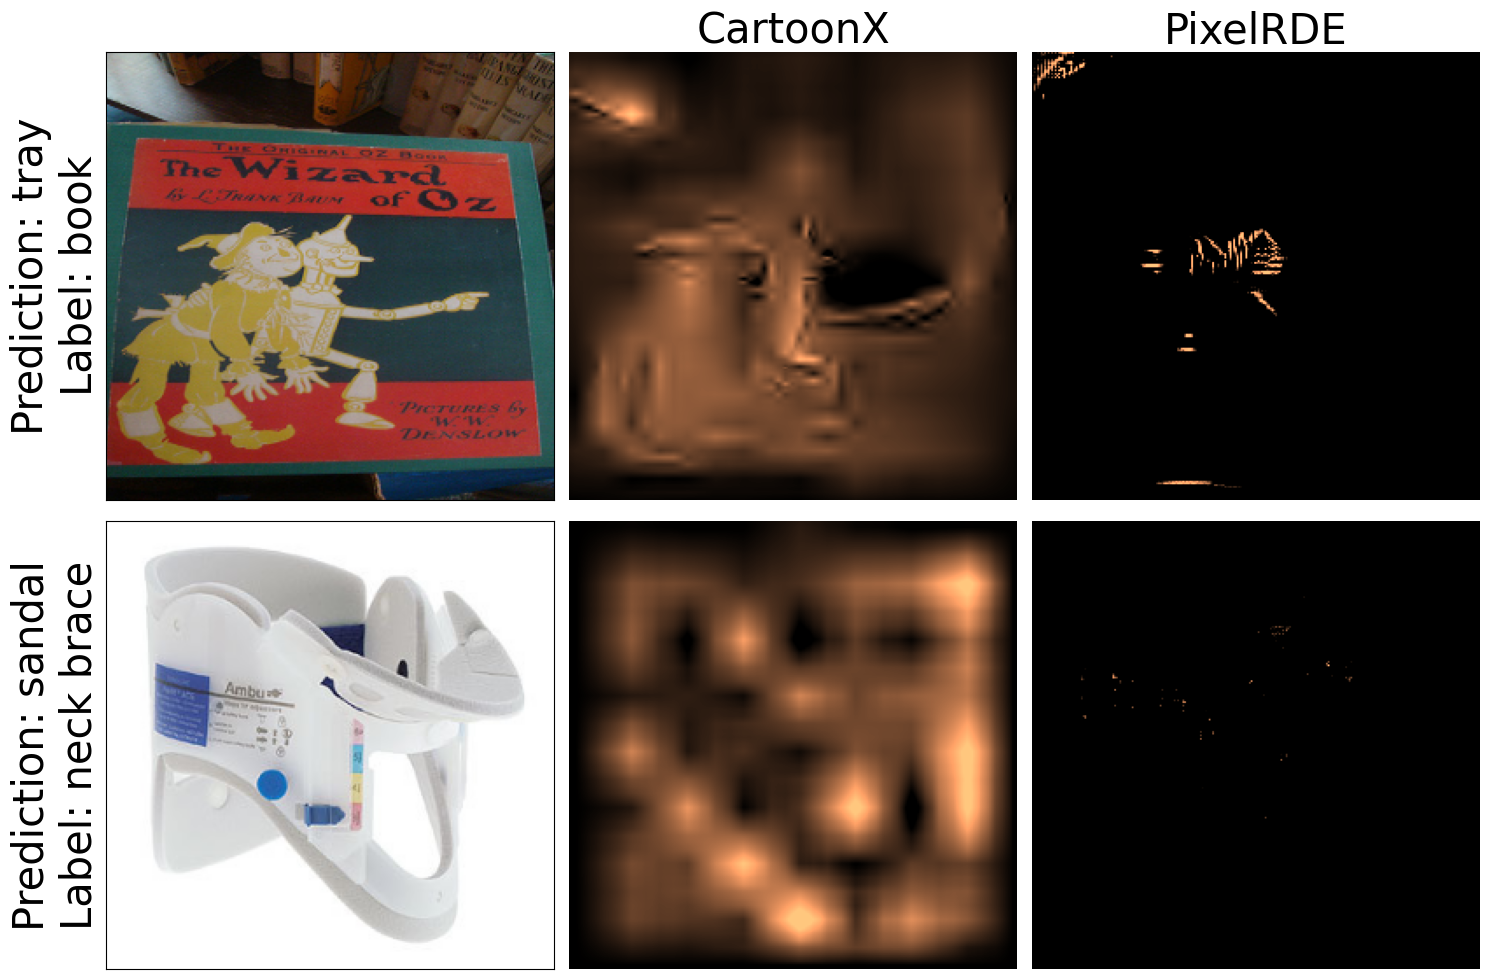
\includegraphics[width=50mm]{images/model_bad_x_bad.png}
    \end{tabular}
    \caption{Examples of misclassifications where CartoonX provides a useful explanation for further investigation (left) and where CartoonX fails at providing a useful explanation (right).}
    \label{fig:model_bad}
\end{figure}

Fig.~\ref{fig:model_bad} shows instances where the model fails and CartoonX either indicates potential reasons (left) or fails to deliver an interpretable explanation (right).
The left images show how the outlines of the objects resemble objects of other classes, giving engineers a chance to adapt their models. 
Pixel RDE cannot produce this explanation.
In the right images, neither method provides a useful explanation.

\subsubsection{Quantitative Reproducibility Experiment}

\begin{figure}
    \centering
    \begin{tabular}{@{}c@{}}
        \includegraphics[width=0.32\linewidth]{images/7a.pdf}
    \end{tabular}
    \begin{tabular}{@{}c@{}}
        \includegraphics[width=0.32\linewidth]{images/7b.pdf}
    \end{tabular}
    \begin{tabular}{@{}c@{}}
        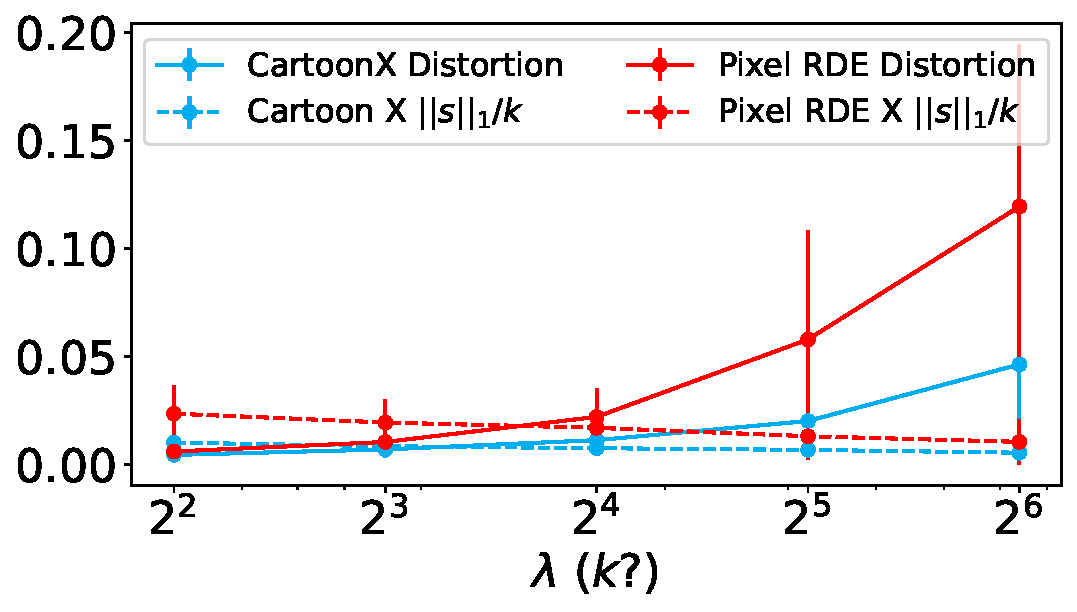
\includegraphics[width=0.32\linewidth]{images/7c.pdf}
    \end{tabular}
    \caption{Distortion as a function of relevant components (left, middle), identified by the explainability method. Distortion as a function of the sparsity settings (right).}
    %In the left image the better method yields the steepest decay. In the middle image the better method yields the steeper increase. In the right image the better method yields smaller distortion values.}
    \label{fig:repro_figure7}
\end{figure}

% CartoonX achieves lower distortion in the model output, using fewer coefficients than Pixel RDE.
The original authors claimed that CartoonX achieves lower distortion in the model output while using fewer coefficients than other state‐of‐the‐art methods.
%While the quantitative experiments do not fully align with the corresponding experiments conducted by the original authors (Fig.~7 in \cite{cartoonX}), the overall message confirms this claim.
Fig.~\ref{fig:repro_figure7} shows three qualitative evaluations of CartoonX vs. Pixel RDE.
The left-most plot depicts the rate-distortion curve when keeping the most relevant coefficients while randomizing the others. The relevance corresponds to the associated mask value.
A good explanation yields a steep decrease in the distortion for low rates, as few coefficients are necessary to classify the image consistently.
The middle plot shows the rate-distortion curve when randomizing the most relevant coefficients while keeping the others.
A good explanation induces a sharp initial increase.
The right-most plot shows the distortion as a function of the sparsity-enforcing hyperparameter $\lambda k$.
A suitable explanation constitutes a compromise between low distortion and high sparsity.
%The better explanation yields lower distortion for a given $\lambda k$.
Across all subexperiments, CartoonX matches or outperforms Pixel RDE.

The exact results diverge in three slight ways from Fig.~7 in the original paper.
First, the steep decrease for low rates of non-randomized components for CartoonX and Pixel RDE (solid lines, left plot) differs from the original figure in terms of magnitude (it drops to $0.25$ in ours vs. $0.45$ in \cite{cartoonX}).
Even though the drop is steeper in our reproduction, the general result stays the same.
They indicate that the most relevant components are equally important for CartoonX and Pixel RDE initially. 
Second, we observe a slight increase of distortion for both methods after the initial drop, whereas in the original paper the distortion dropped more continuously.
Since we mostly care about the relative initial drop, we still confirm the conclusion that CartoonX is superior according to this metric.
Third, the obtained non-sparsity values when varying $\lambda k$ (dashed lines, right plot) are significantly lower, despite the curves' general shape being similar.
%Even though the exact plots from Fig.~7 in the original paper~\cite{cartoonX} diverge from ours (Fig.~\ref{fig:repro_figure7}), the overall message is still the same: \textit{CartoonX outperforms Pixel RDE by all quantitative measures used by the original authors.}
Notwithstanding, our results are in line with the claims made by the original authors, as the non-sparsity value values for Pixel RDE (red) are always higher than for CartoonX (blue).
%CartoonX produces piece-wise smooth explanations, which are more intuitive to interpret for humans than pixel-sparse explanations. We conclude that the explanations usually give valuable insights for engineers and users alike.



\subsection{Results beyond original paper}
%Often papers don't include enough information to fully specify their experiments, so some additional experimentation may be necessary. For example, it might be the case that batch size was not specified, and so different batch sizes need to be evaluated to reproduce the original results. Include the results of any additional experiments here. Note: this won't be necessary for all reproductions.
 
\subsubsection{Model Agnosticism Experiment} 
%With this setup (experimental setup 3), we tried to verify the third claim of the authors, i.e., the claim that CartoonX is model agnostic.
%The authors' claim that CartoonX is model-agnostic was examined by means of the model agnosticism experiment where CartoonX was run with another kind of classifier, namely a ViT.
We examine the claim that CartoonX is model-agnostic by running CartoonX on a ViT.
Fig.~\ref{fig:vit_res} shows four resulting sample explanations, qualitatively comparing the original image, CartoonX for CNN, CartoonX for ViT, and the attention rollout. For a fair comparison, only the cases where the CNN and the ViT predicted the same and the correct class were considered. 
On the left side in Fig. \ref{fig:vit_res}, two examples are shown where both CartoonX for CNN and CartoonX for ViT provide a helpful explanation.
%, identifying the pelican (top) and the middle of the dam (bottom).
Moreover, for both images, this coincides approximately with the attention rollout.
%, approximately marking the same areas as having high attention values. %For the dam image, the CartoonX for the ViT is even more precise than the attention rollout
% The cartoonX is even more precise than the attention rollout 
On the right side in Fig. \ref{fig:vit_res}, two examples are shown where CartoonX for ViT provides a very sparse, almost completely black, explanation while CartoonX for CNN does not. 
For both images, the attention rollout is not sparse and mainly marks the upper background of the image as having high attention values, also not providing an interpretable reason for the models' decision. %For the saxophone (bottom right), both the CartoonX explanation for the ViT and the attention rollout focus on the same non-subject areas.   

In Fig.~\ref{fig:ViT-Quantitative}, both curves for CartoonX (with CNN and ViT) follow a similar shape.
The distortion achieved with the ViT drops sharply when randomizing all but the most relevant components (left) and increases sharply when randomizing the most relevant components (right).
This is in accordance with the findings for CartoonX on CNNs.

\begin{figure}
    \begin{tabular}{@{}c@{}}
        \includegraphics[width=65mm]{images/good_vit_res.png}
    \end{tabular}
    \begin{tabular}{@{}c@{}}
        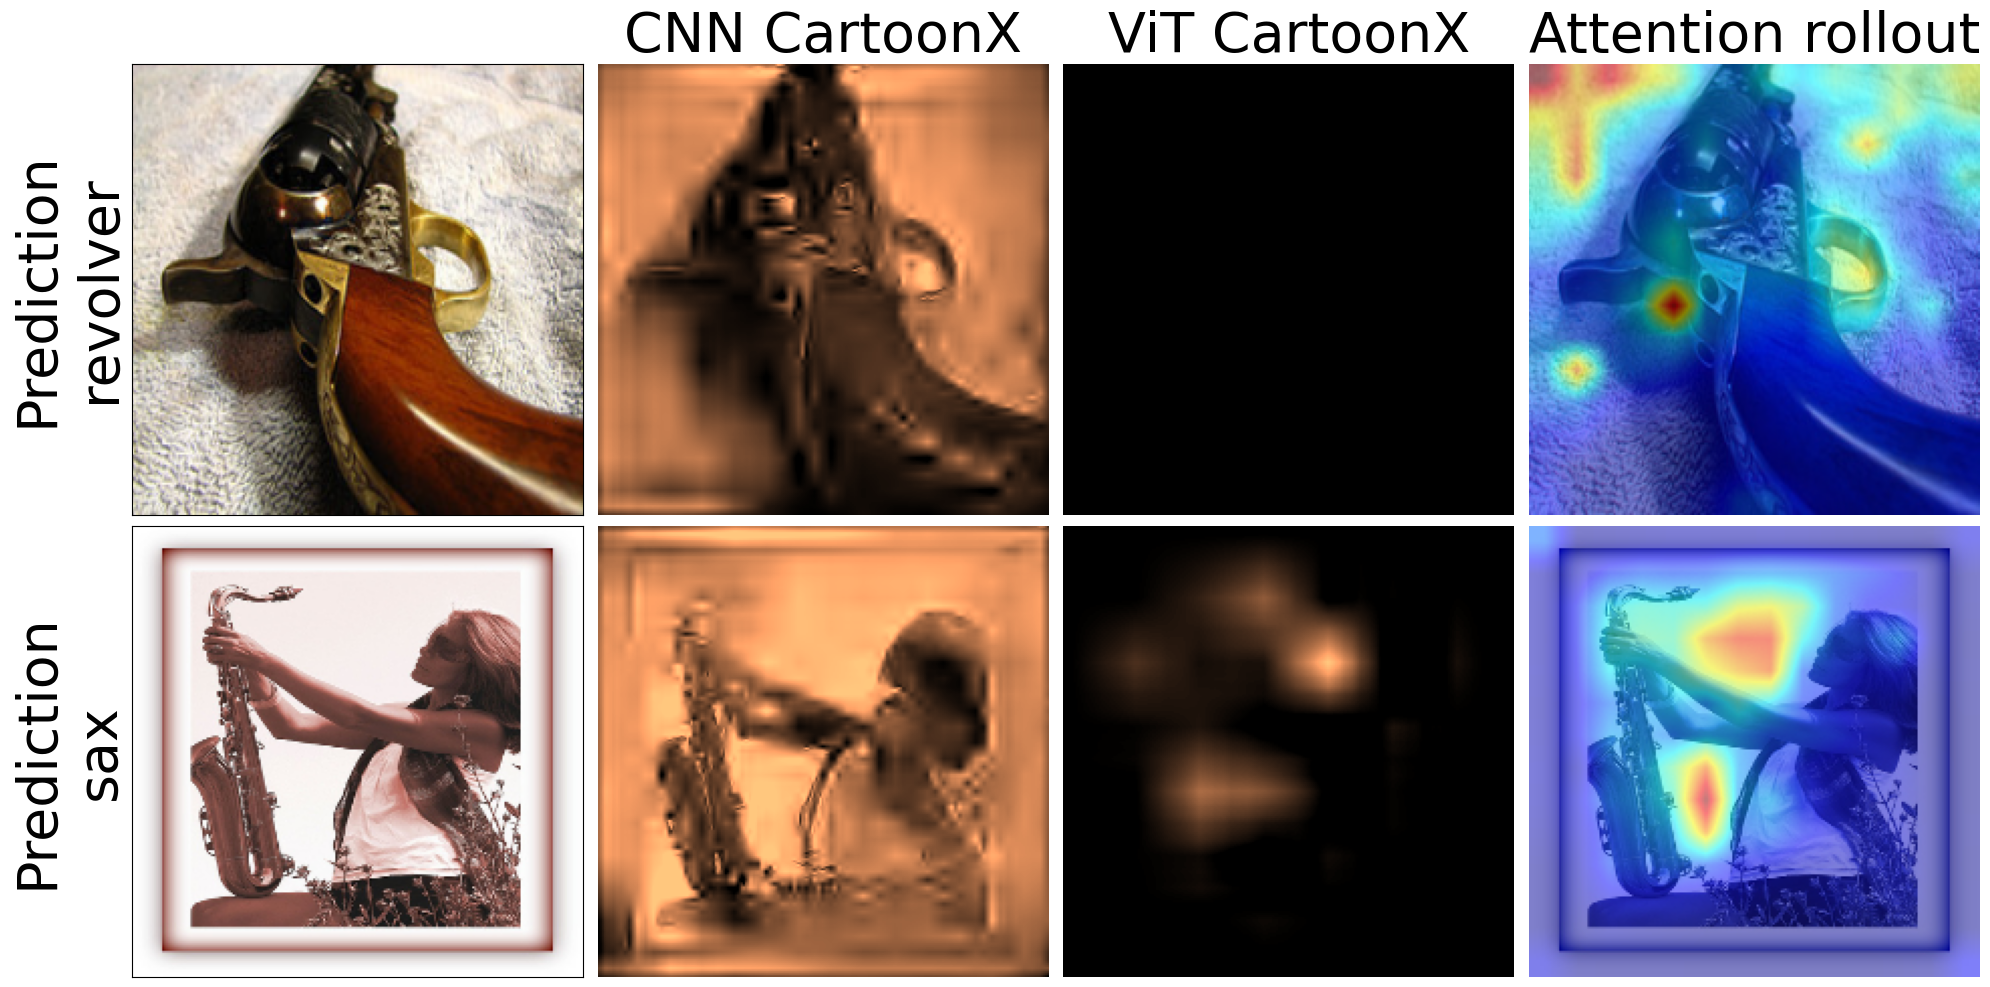
\includegraphics[width=65mm]{images/bad_vit_res.png}
    \end{tabular}
    \caption{Cases where CartoonX provides a useful explanation for both CNN and ViT (left) and cases where CartoonX (ViT) and the attention rollout do not provide an intelligible explanation of the model's decision (right).}
    \label{fig:vit_res}
\end{figure}

\begin{figure}[htb]
    \centering
    \begin{tabular}{@{}c@{}}
        \includegraphics[width=0.32\linewidth]{images/ViT-Quantitative-a}
    \end{tabular}
    \begin{tabular}{@{}c@{}}
        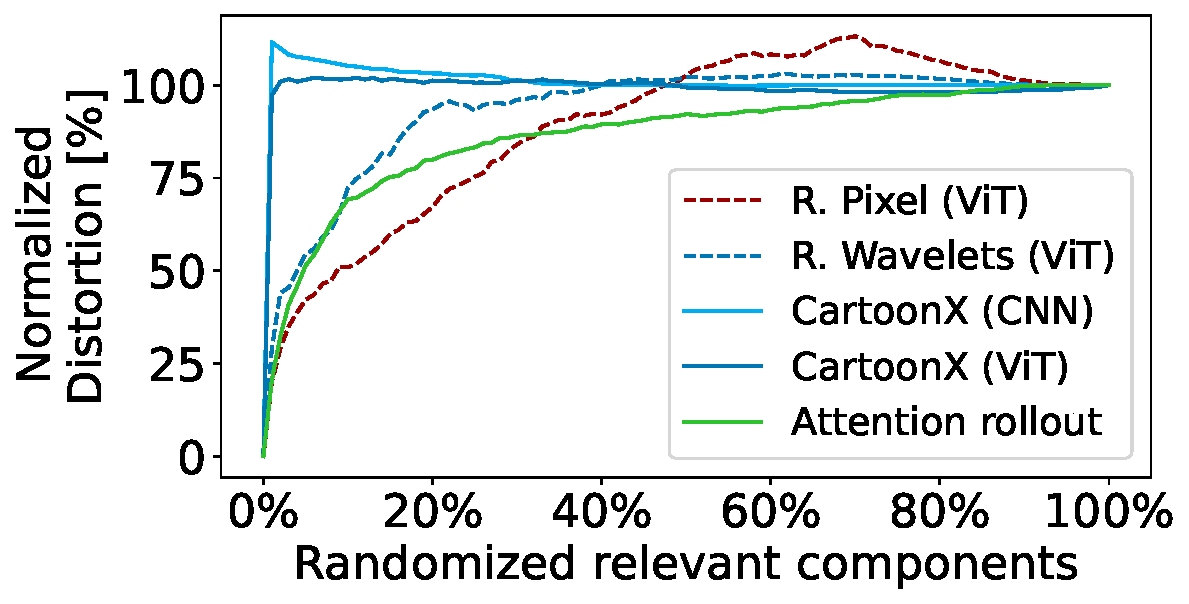
\includegraphics[width=0.32\linewidth]{images/ViT-Quantitative-b}
    \end{tabular}
    \caption{Normalized distortion as a function of relevant components, identified by CartoonX and the attention rollout (random pixels/wavelet coefficients, and attention rollout as benchmark).}
    \label{fig:ViT-Quantitative}
\end{figure}

% ToDo integrate into previous paragraph
%By comparing CartoonX to the attention mask of the transformer model, we conclude that both methods mostly point to the same areas. Nonetheless, it should be noted that uninterpretable results of one method usually correspond to uninterpretable results of the other, resulting in some overlap and redundancy in explanations.
Overall, when regarding the results of all $100$ images, the majority of ViT CartoonX explanations are sparser and more sensitive to the choice of $\lambda k$ compared to their CNN counterparts.
Furthermore, in Fig.~\ref{fig:ViT-Quantitative}, both a sharper initial drop (left) and increase (right) can be observed for the CNN compared to the ViT, indicating marginally worse performance for ViTs.
While the CNN-based explanations are marginally superior, the correct identification of relevant components in the ViT case is still apparent.
Hence, our findings mostly support the claim of model agnosticism.
%TODO note on how attention rollout stacks up against other methods?
 

\subsubsection{Runtime Efficiency Experiment}
The original authors proposed using neural networks to predict an initialization for the deletion mask to speed up their algorithm's runtime.
We investigated whether simple heuristics could already produce a good initialization suitable for that purpose.

\begin{figure}[htb]
    \centering
    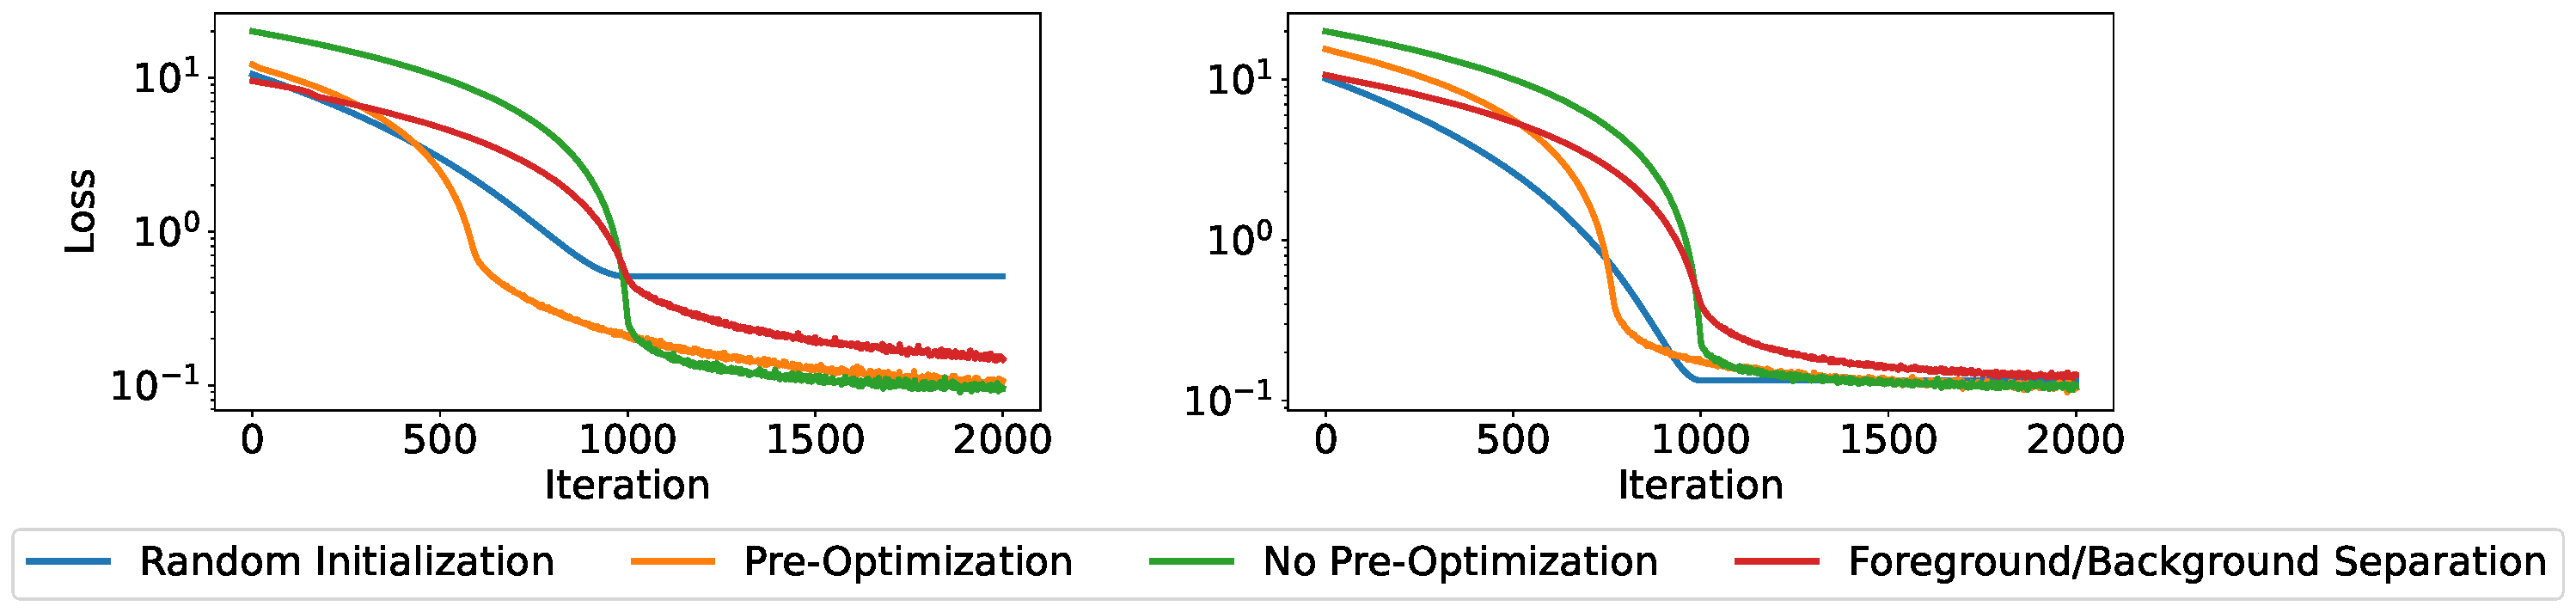
\includegraphics[width=120mm]{images/loss_curves_speedup.pdf}
    \caption{Comparing the loss curves of the CartoonX optimization algorithm with different deletion mask initializations for two different images.}
    \label{fig:speed}
\end{figure}

Fig.~\ref{fig:speed} shows the loss curves for different initialization strategies for two sample images.
While the preoptimized mask leads to faster initial convergence, the loss curve flattens quickly.
Before qualitatively good convergence, the preoptimization and normal initialization curves reunite again.
It is important to note that the slight differences in loss after around $1000$ iterations make a notable difference in the explanation's quality.
The foreground segmentation did not yield beneficial results due to the final loss being too high compared to other methods.
Lastly, random initialization was tested, which led to unrobust results.

These outcomes indicate that more complex approaches might be required to obtain the desired speedup. Such an approach could be to utilize neural networks to predict the initial deletion mask. 
Furthermore, our results suggest that these networks must act risk averse, i.e., using a less sparse mask rather than blocking out many wavelet coefficients.
The reason for that is that unrobust results were observed for any mask, which was already made too sparse at initialization.

\subsection{Critique of our methods}
For all experiments, a value for $\lambda k$ was qualitatively, thus somewhat subjectively, chosen.
Being limited to running the experiments on a small subset of ImageNet, consisting of $100$ random images from distinct classes, the samples were not entirely randomly chosen (no duplicate classes were included).
Nonetheless, this method ensures more diversity, especially in the qualitative analysis.
The lack of a decisive measure to define convergence complicated the determination of a suitable number of training iterations.
Furthermore, it led to a rather vague interpretation of what can be considered a speedup of the algorithm.
Lastly, it should be noted that the attention mask, used for comparison in the ViT experiment, is not explicitly designed to serve as an explanation~\cite{jain2019attention_not_explanation}.


\section{Reproducibility review} \label{sec:over} 
%Give your judgement on if your experimental results support the claims of the paper. Discuss the strengths and weaknesses of your approach - perhaps you didn't have time to run all the experiments, or perhaps you did additional experiments that further strengthened the claims in the paper.

%The experimental results from Section~\ref{sec:results} are primarily in line with the claims made by the original authors.
%CartoonX produces piece-wise smooth explanations, which are more intuitive to interpret for humans than pixel-sparse explanations.
%We conclude that the explanations usually give valuable insights for engineers and users alike.

% Furthermore, we show that CartoonX yields less distortion for the same number of relevant coefficients included in the image and also for different values of $\lambda k$.
% Even though the exact plots from Fig.~7 in the original paper~\cite{cartoonX} diverge from ours (see Fig.~\ref{fig:repro_figure7}), the overall message is still the same: \textit{CartoonX outperforms Pixel RDE by all quantitative measures used by the original authors.}

%The exact plots from Fig.~7 in the original paper~\cite{cartoonX} diverge from ours (see Fig.~\ref{fig:repro_figure7}) in three ways. First, the size of the steep decrease for low rates of non-randomized components (left plot) is similar between CartoonX and Pixel RDE but different compared to the original implementation. This indicates that the most relevant components are equally important between CartoonX and Pixel RDE. Second, the distortion converges to $\sim0.5$, considerably lower than the value of $\sim0.65$ from the original implementation. However, the difference in used images can explain this, as the exact distortion varies considerably per image. Finally, the distortion values when varying $\lambda k$ (right plot) are significantly lower, although the general shape is similar. Even though the exact plots from Fig.~7 in the original paper~\cite{cartoonX} diverge from ours (Fig.~\ref{fig:repro_figure7}), the overall message is still the same: \textit{CartoonX outperforms Pixel RDE by all quantitative measures used by the original authors.}

%We demonstrated that CartoonX can also be used in conjunction with a ViT, thus substantiating the agnosticism claim.
%By comparing CartoonX to the attention mask of the transformer model, we conclude that both methods mostly point to the same areas.
%We propose the complementary use of attention masks and CartoonX to gain model insights.
%The quantitative results underline that CartoonX tends to exhibit better performance for the CNN. Notwithstanding, the correct identification of relevant components by the ViT counterpart compared to the random baselines is apparent. 
%Nonetheless, it should be noted that uninterpretable results of one method usually correspond to uninterpretable results of the other, resulting in some overlap and redundancy in explanations.

%Lastly, the conducted experiments indicate that simple solutions are ineffective in reducing the runtime performance and that more complex approaches might be required to obtain the desired speedup. Such an approach could be to utilize neural networks to predict the initial deletion mask. 
%Furthermore, our results suggest that these networks must act risk averse, i.e., using a less sparse mask rather than blocking out many wavelet coefficients.
%The reason being that unrobust results were observed for any mask that was already made too sparse at initialization.

\subsection{What was easy}
%Give your judgement of what was easy to reproduce. Perhaps the authors' code is clearly written and easy to run, so it was easy to verify the majority of original claims. Or, the explanation in the paper was really easy to follow and put into code. 

%Be careful not to give sweeping generalizations. Something that is easy for you might be difficult to others. Put what was easy in context and explain why it was easy (e.g. code had extensive API documentation and a lot of examples that matched experiments in papers). 
The original paper had an extensive explanation of the background of CartoonX, both mathematically and intuitively. Moreover, they provided an article on wavelets\footnote{\url{https://julheg.github.io/waveletexplainability/}} for explainability, making it easier to understand. 
The provided implementation was well-documented and ran trouble-free. Therefore, the qualitative experiments were easy to replicate, by merely executing the code on different images and analyzing the results. Furthermore, it was straightforward to extend their code, as it was well-modularized.

\subsection{What was difficult}
%List part of the reproduction study that took more time than you anticipated or you felt were difficult. 
%Be careful to put your discussion in context. For example, don't say "the maths was difficult to follow", say "the math requires advanced knowledge of calculus to follow". 
% which lambda values for which figure? 
Recreating Fig.~\ref{fig:repro_figure7} was difficult due to uncertainties of which hyperparameters ($\lambda k$, number of iterations) or models were used.
Furthermore, since there is no convergence criterion provided for CartoonX, it was difficult to get an intuition for the loss curves. 
Lastly, the original paper did not specify the exact subset of ImageNet images.
This necessitates a more general evaluation but hinders direct comparisons between the original paper and ours.

\subsection{Communication with original authors}
%Document the extent of (or lack of) communication with the original authors. To make sure the reproducibility report is a fair assessment of the original research we recommend getting in touch with the original authors. You can ask authors specific questions, or if you don't have any questions you can send them the full report to get their feedback before it gets published.

We inquired about clarifications on the values used for $\lambda k$ for the qualitative analysis.
The authors reported that they used variant values for different images.
Nonetheless, only the same value for each image was used in this study to ensure consistency between different images.
We further enquired about the $\lambda k$ values used to recreate Fig.~7(a) and (b) of the original paper.
Unfortunately, confirmation regarding these values was not provided.
Overall, the authors were quick to respond and were open to answer most of the questions as detailed as possible.


\section{Conclusion}\label{sec:conclusion}

CartoonX is a valuable explanation method that yields piece-wise smooth explanations.
We found this explanation style to be more interpretable than pixel-sparse explanations.
It works well for CNNs and, for the most part, also yields good explanations for ViTs.
Overall, it is a valuable addition to the ever-growing set of explanation methods available to deep learning researchers, engineers, and users.

Future research could explore how to define a decisive measure of convergence for CartoonX.
Such a measure would help evaluate the effectiveness of smart initialization strategies to improve runtime. 
Specifically, we see potential to investigate neural networks for predicting initial deletion masks, as previously discussed and already suggested by the original authors.
Lastly, considering a wider range of image-specific $\lambda k$ values, especially for the ViT, might improve the overall quality of the explanations.
%Lastly, we propose to recreate Fig.~7c from the original paper for the ViT; which we left out due to time constraints.
